\documentclass{article}
\usepackage{tikz, comment}
\usepackage{pifont}
\usepackage{fontspec, pgfplots}
\usetikzlibrary{arrows, decorations.markings, decorations.pathreplacing}
\begin{comment}
:Title: Not defined yet
:Tags: triple (scalar) product;adjugate, classical adjoint;properties of equality, equation rules;set;element of a set
:Prob: 0.5356;0.5272;0.4871;0.4789;0.4737
:Author: Prof.Hu Ji-shan, HKUST
:Slug: No name yet

Description Here.........
\end{comment}
\begin{document}\centering 

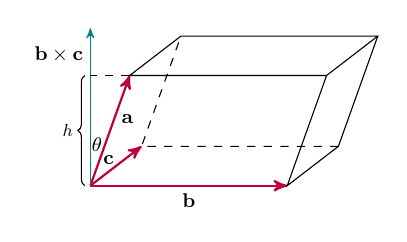
\begin{tikzpicture}[>=latex,xscale=.5*1, yscale=.5*1][font=\sf\small] 

\draw[purple, thick, ->, >=stealth'] (0, 0) -- (1, 2.8) node[black, right, midway, pos=0.6, xshift=0, yshift=0, scale=0.8]{${\bf a}$};

\draw[purple, thick, ->, >=stealth'] (0, 0) -- (5, 0) node[black, below, midway, pos=0.5, xshift=0, yshift=0, scale=0.8]{${\bf b}$};

\draw[purple, thick, ->, >=stealth'] (0, 0) -- (1.3, 1) node[black, left, midway, pos=0.5, xshift=2, yshift=2, scale=0.8]{${\bf c}$};

\draw (1, 2.8)--++(5, 0)--++(1.3, 1)--++(-5, 0)--++(-1.3, -1);
\draw (6, 2.8)--++(-1, -2.8)--++(1.3, 1)--++(1, 2.8);

\draw[dashed] (6.3, 1)--++(-5, 0)--++(1, 2.8);

\draw[teal, ->, >=stealth'] (0, 0) -- (0, 4) node[black, left, midway, pos=0.8, xshift=0, yshift=2, scale=0.8]{${\bf b\times c}$};

\draw[dashed] (1, 2.8)--(0, 2.8);

\draw [decoration={brace,raise=2},decorate, yshift=0] 
(0, 0)--(0, 2.8) node[black, left, midway, pos=0.5, xshift=-4, yshift=0, scale=0.7]{$h$};

\node[xshift=2.4, yshift=15, scale=0.8] at (0,0) {$\theta$};

\end{tikzpicture}
\end{document}